\documentclass[tikz,border=8pt]{standalone}
\usepackage{amsmath,amssymb}
\usetikzlibrary{arrows.meta,calc,decorations.markings,patterns,positioning}

\begin{document}
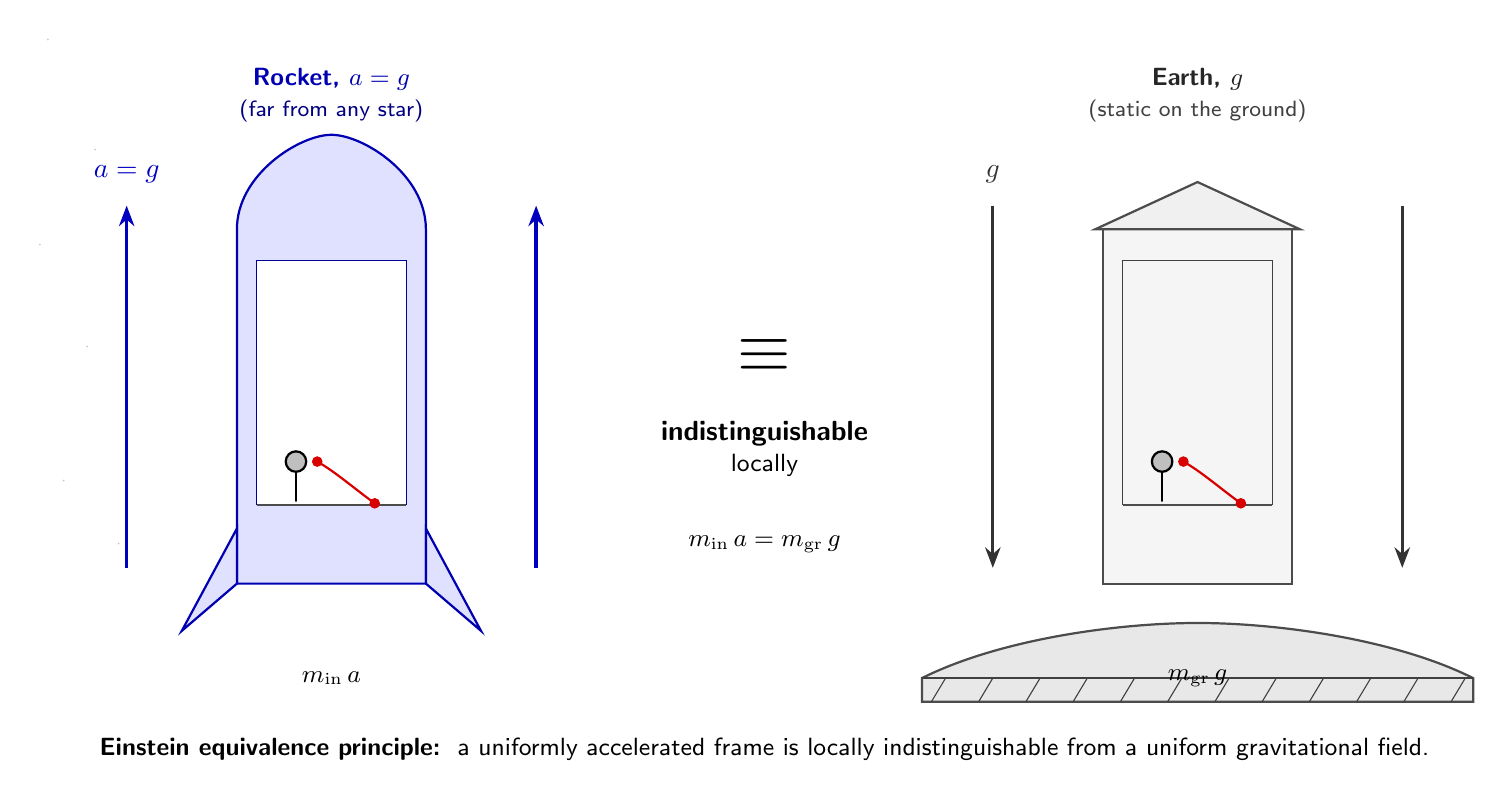
\begin{tikzpicture}[
    >={Stealth[length=2.6mm]},
    font=\sffamily\small,
    rocketBody/.style={draw=blue!70!black,fill=blue!12,thick},
    rocketWindow/.style={draw=blue!60!black,fill=white,thin},
    earthArc/.style={draw=gray!60!black,fill=gray!18,thick},
    person/.style={draw=black,fill=gray!50,thick,line cap=round},
    ballPath/.style={red!85!black,thick},
    ballDot/.style={fill=red!85!black,draw=red!85!black},
    bigArrow/.style={->,very thick,blue!75!black},
    bigArrowG/.style={->,very thick,gray!40!black},
    eqSym/.style={font=\sffamily\bfseries\Huge,black},
    boxLabel/.style={font=\sffamily\small,align=center}
]

% =====================================================
% LEFT SCENE: Rocket far from any star, accelerating up at a = g
% =====================================================
\begin{scope}[shift={(0,0)}]

  % Outer space dotted background hint (sparse stars)
  \foreach \sx/\sy in {-3.6/4.4, -3.0/3.0, -3.7/1.8, -3.1/0.5, -3.4/-1.2, -2.7/-2.0}{
    \node[font=\tiny,gray!50] at (\sx,\sy) {$\cdot$};
  }

  % Rocket body: a tall capsule with rounded top
  % Body: rectangle 2.4 x 5
  \draw[rocketBody] (-1.2,-2.5) -- (-1.2,2.0)
                    .. controls (-1.2,2.7) and (-0.4,3.2) .. (0,3.2)
                    .. controls (0.4,3.2) and (1.2,2.7) .. (1.2,2.0)
                    -- (1.2,-2.5) -- cycle;

  % Fins
  \draw[rocketBody] (-1.2,-2.5) -- (-1.9,-3.1) -- (-1.2,-1.8) -- cycle;
  \draw[rocketBody] (1.2,-2.5) -- (1.9,-3.1) -- (1.2,-1.8) -- cycle;

  % Window for the cabin (interior view)
  \draw[rocketWindow] (-0.95,-1.5) rectangle (0.95,1.6);

  % Floor inside cabin
  \draw[gray!60!black,thick] (-0.95,-1.5) -- (0.95,-1.5);

  % Person inside (head, body, legs)
  \fill[person] (-0.45,-0.95) circle (0.13);
  \draw[person] (-0.45,-1.08) -- (-0.45,-1.45);

  % Ball trajectory: from hand at (-0.18,-0.95) to floor, parabolic
  % Using a control point that mimics free-fall arc
  \draw[ballPath] (-0.18,-0.95)
                 .. controls (0.05,-1.08) and (0.30,-1.30) .. (0.55,-1.48);
  % Initial ball position
  \node[ballDot,circle,inner sep=1.2pt] at (-0.18,-0.95) {};
  % Final ball position (on floor)
  \node[ballDot,circle,inner sep=1.2pt] at (0.55,-1.48) {};

  % Big upward acceleration arrow OUTSIDE rocket
  \draw[bigArrow] (-2.6,-2.3) -- (-2.6,2.3);
  \node[blue!75!black,font=\sffamily\bfseries] at (-2.6,2.7) {$a = g$};

  % Tick: another arrow on right showing acceleration
  \draw[bigArrow] (2.6,-2.3) -- (2.6,2.3);

  % Scene title
  \node[boxLabel,blue!70!black] at (0,3.9) {\textbf{Rocket, $a=g$}};
  \node[boxLabel,blue!50!black,font=\sffamily\footnotesize] at (0,3.5) {(far from any star)};

  % Inertial law: m_in * a
  \node[boxLabel] at (0,-3.7) {$m_{\rm in}\,a$};

\end{scope}

% =====================================================
% CENTER: equivalence symbol and "indistinguishable" label
% =====================================================
\begin{scope}[shift={(5.5,0)}]
  \node[eqSym] at (0,0.4) {$\equiv$};
  \node[boxLabel,font=\sffamily\bfseries] at (0,-0.6)
    {indistinguishable};
  \node[boxLabel,font=\sffamily\small] at (0,-1.0)
    {locally};
  % Arrow tying both sides: equation
  \node[boxLabel,font=\sffamily\small] at (0,-2.0)
    {$m_{\rm in}\,a = m_{\rm gr}\,g$};
\end{scope}

% =====================================================
% RIGHT SCENE: Stationary cabin on Earth's surface in gravity g
% =====================================================
\begin{scope}[shift={(11,0)}]

  % Earth's curve (a thick arc at the bottom)
  % Earth as part of a big circle, just showing the top arc segment.
  \draw[earthArc,fill=gray!18] (-3.5,-3.7)
       .. controls (-2.5,-3.2) and (-1.0,-3.0) .. (0,-3.0)
       .. controls (1.0,-3.0) and (2.5,-3.2) .. (3.5,-3.7)
       -- (3.5,-4.0) -- (-3.5,-4.0) -- cycle;

  % Surface ground line
  \draw[gray!50!black,thick] (-3.5,-3.7) -- (3.5,-3.7);
  % Hatching on ground
  \foreach \gx in {-3.2,-2.6,-2.0,-1.4,-0.8,-0.2,0.4,1.0,1.6,2.2,2.8,3.4}{
     \draw[gray!50!black,thin] (\gx,-3.7) -- (\gx-0.18,-4.0);
  }

  % Cabin (rectangular, identical interior dimensions to rocket cabin)
  % Outer wall
  \draw[gray!60!black,fill=gray!8,thick] (-1.2,-2.5) rectangle (1.2,2.0);
  % Roof (slight pitched look)
  \draw[gray!60!black,fill=gray!12,thick] (-1.3,2.0) -- (0,2.6) -- (1.3,2.0) -- cycle;

  % Interior window/frame
  \draw[gray!50!black,thin] (-0.95,-1.5) rectangle (0.95,1.6);

  % Floor inside cabin
  \draw[gray!60!black,thick] (-0.95,-1.5) -- (0.95,-1.5);

  % Person inside
  \fill[person] (-0.45,-0.95) circle (0.13);
  \draw[person] (-0.45,-1.08) -- (-0.45,-1.45);

  % Ball trajectory: identical to left scene
  \draw[ballPath] (-0.18,-0.95)
                 .. controls (0.05,-1.08) and (0.30,-1.30) .. (0.55,-1.48);
  \node[ballDot,circle,inner sep=1.2pt] at (-0.18,-0.95) {};
  \node[ballDot,circle,inner sep=1.2pt] at (0.55,-1.48) {};

  % Big downward gravity arrow OUTSIDE cabin
  \draw[bigArrowG] (-2.6,2.3) -- (-2.6,-2.3);
  \node[gray!40!black,font=\sffamily\bfseries] at (-2.6,2.7) {$g$};

  \draw[bigArrowG] (2.6,2.3) -- (2.6,-2.3);

  % Scene title
  \node[boxLabel,gray!30!black] at (0,3.9) {\textbf{Earth, $g$}};
  \node[boxLabel,gray!50!black,font=\sffamily\footnotesize] at (0,3.5) {(static on the ground)};

  % Gravitational law: m_gr * g
  \node[boxLabel] at (0,-3.7) {$m_{\rm gr}\,g$};

\end{scope}

% =====================================================
% Bottom annotation: principle name
% =====================================================
\node[font=\sffamily\small,align=center] at (5.5,-4.6)
  {\textbf{Einstein equivalence principle:}\ \ a uniformly accelerated frame is
   locally indistinguishable from a uniform gravitational field.};

\end{tikzpicture}
\end{document}
